\section{Motivation}
\label{sec:motivation}

\dsnvm\ is motivated by three datacenter trends: 
emerging hardware \nvm\ technologies, 
modern data-intensive applications' data sharing, persistence, and reliability needs, 
and the availability of fast datacenter network.

\subsection{Persistent Memory and PM Apps}
Next-generation non-volatile memories ({\em NVMs}), 
such as 3DXpoint~\cite{Intel3DXpoint}, phase change memory ({\em PCM}),
spin-transfer torque magnetic memories ({\em STTMs}), and the memristor
will provide byte addressability, persistence, and latency that is within 
an order of magnitude of 
DRAM~\cite{hosomi2005novel,Lee10-pcmquest,lee2010phase,lee2011fast,qureshi2010morphable,NVMDB,yang2013memristive,Octopus}.
These developments are poised to radically alter the landscape of memory and storage technologies.

NVMs can attach directly to the main memory bus to form Persistent Memory, or \nvm. 
If applications want to exploit all the low latency and byte-addressability benefits of \nvm,
they should directly access it via memory load and store instructions without any software 
overheads~\cite{Coburn11-ASPLOS,Volos11-ASPLOS,Zhang15-Mojim,Memory-Persistency,Kamino-EuroSys17,pmxact-asplos16} 
(we call this model {\em durable in-memory computation}),
rather than accessing it via a file system~\cite{sosp09:bpfs,Dragojevic14-NSDI,Dulloor14-EuroSys,Xiaojian11-SC,HiNFS-Eurosys16,Octopus}.

{
\begin{figure}[th]
\begin{center}
\centerline{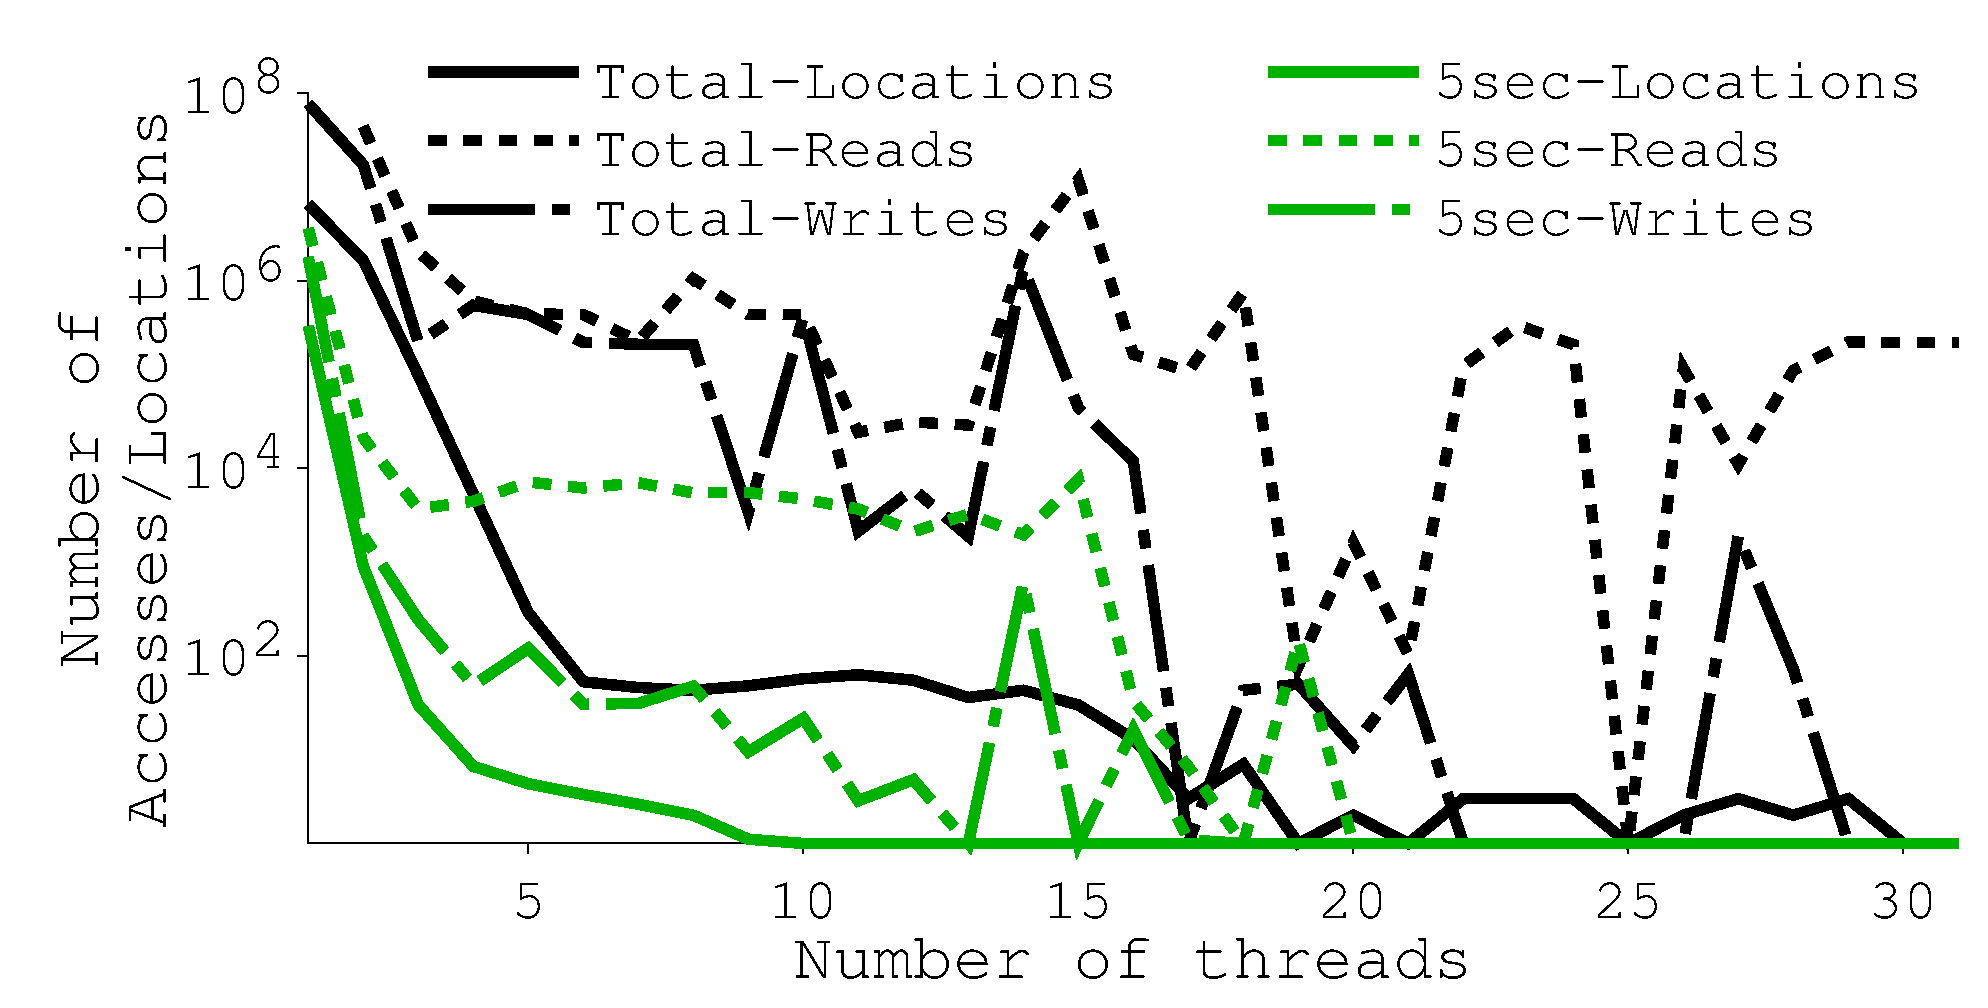
\includegraphics[width=0.4\textwidth]{Figures/g_plot_pagerank_average.pdf}}
\vspace{-0.15in}
\mycaption{fig-pagerank}{PowerGraph Sharing Analysis.}
{
Results of running PageRank~\cite{PageRank} on a Twitter graph~\cite{Kwak10-WWW}.
%Number of PowerGraph Pagerank memory reads and writes that are performed by $N$ threads to a shared location,
%and the number of such shared locations.
Black lines represent total amount of sharing.
Green lines represent sharing within five seconds.
}
\end{center}
\vspace{-0.2in}
\end{figure}
}

Unfortunately, most previous durable in-memory systems were designed for the single-node environment.
With modern datacenter applications' computation scale, 
we have to be able to scale out these single-node \nvm\ systems.

\subsection{Shared Memory Applications}
Modern data-intensive applications increasingly need
to access and share vast amounts of data fast. 
We use PIN~\cite{Luk05-PLDI} to collect memory access traces of two popular data-intensive applications, 
TensorFlow~\cite{TensorFlow} and PowerGraph~\cite{Gonzalez12-OSDI}.
Figures~\ref{fig-pagerank} and \ref{fig-tensorflow} show the total number of reads and writes performed to the same memory location 
by $N$ threads and the amount of these shared locations.
There are a significant amount of shared read accesses in these applications,
especially across a small set of threads.
We further divided the memory traces into smaller time windows 
and found that there is still a significant amount of sharing, 
indicating that many shared accesses occur at similar times. 

Distributed Shared Memory ({\em \dsm}) takes the shared memory concept a step further 
by organizing a pool of machines into a globally shared memory space.
Researchers and system builders have developed a host of software and hardware \dsm\ systems in the past few 
decades~\cite{Bennett90-PPOPP,Bisiani90-ISCA,Black89-COMPCON,Delp:1988:AIM:59505,Fleisch89-SOSP,Gibbons91-SPAA,Kontothanassis97-ISCA,Lo94-AC,Kessler89-ACM,Keleher92-ISCA,Ramachandran91-Wiley,Zhou92-IEEE,Stumm90-IEEE,Stumm90-IPDPS,HLRC,Shasta}.
Recently, there is a new interest in \dsm~\cite{Nelson15-ATC} to support modern data-intensive applications.

However, although DSM scales out shared-memory applications, 
there has been no persistent-memory support for DSM.
DSM systems all had to checkpoint to disks~\cite{Stumm90,Richard93,Neves94}.
Memory persistence
can allow these applications to checkpoint fast and recover fast~\cite{Narayanan12-ASPLOS}.

\subsection{Fast Network and RDMA}
Datacenter network performance has improved significantly over the past decades.
InfiniBand ({\em \ib}) NICs and switches support high bandwidth ranging from 40 to 100\gbps.
Remote Direct Memory Access ({\em RDMA}) technologies that provide low-latency remote memory accesses
have become more mature for datacenter uses in recent years~\cite{FaSST,Dragojevic14-NSDI,Kalia14-SIGCOMM,Guo16-SIGCOMM}.
These network technology advances
make remote-memory-based systems~\cite{Nelson15-ATC,GU17-NSDI,OSDI-Disaggregate,Chen16-EUROSYS,Binnig16-VLDB,Zamanian17-VLDB} more attractive than decades ago.

\subsection{Lack of Distributed PM Support}

{
\begin{figure}[t]
\begin{center}
\centerline{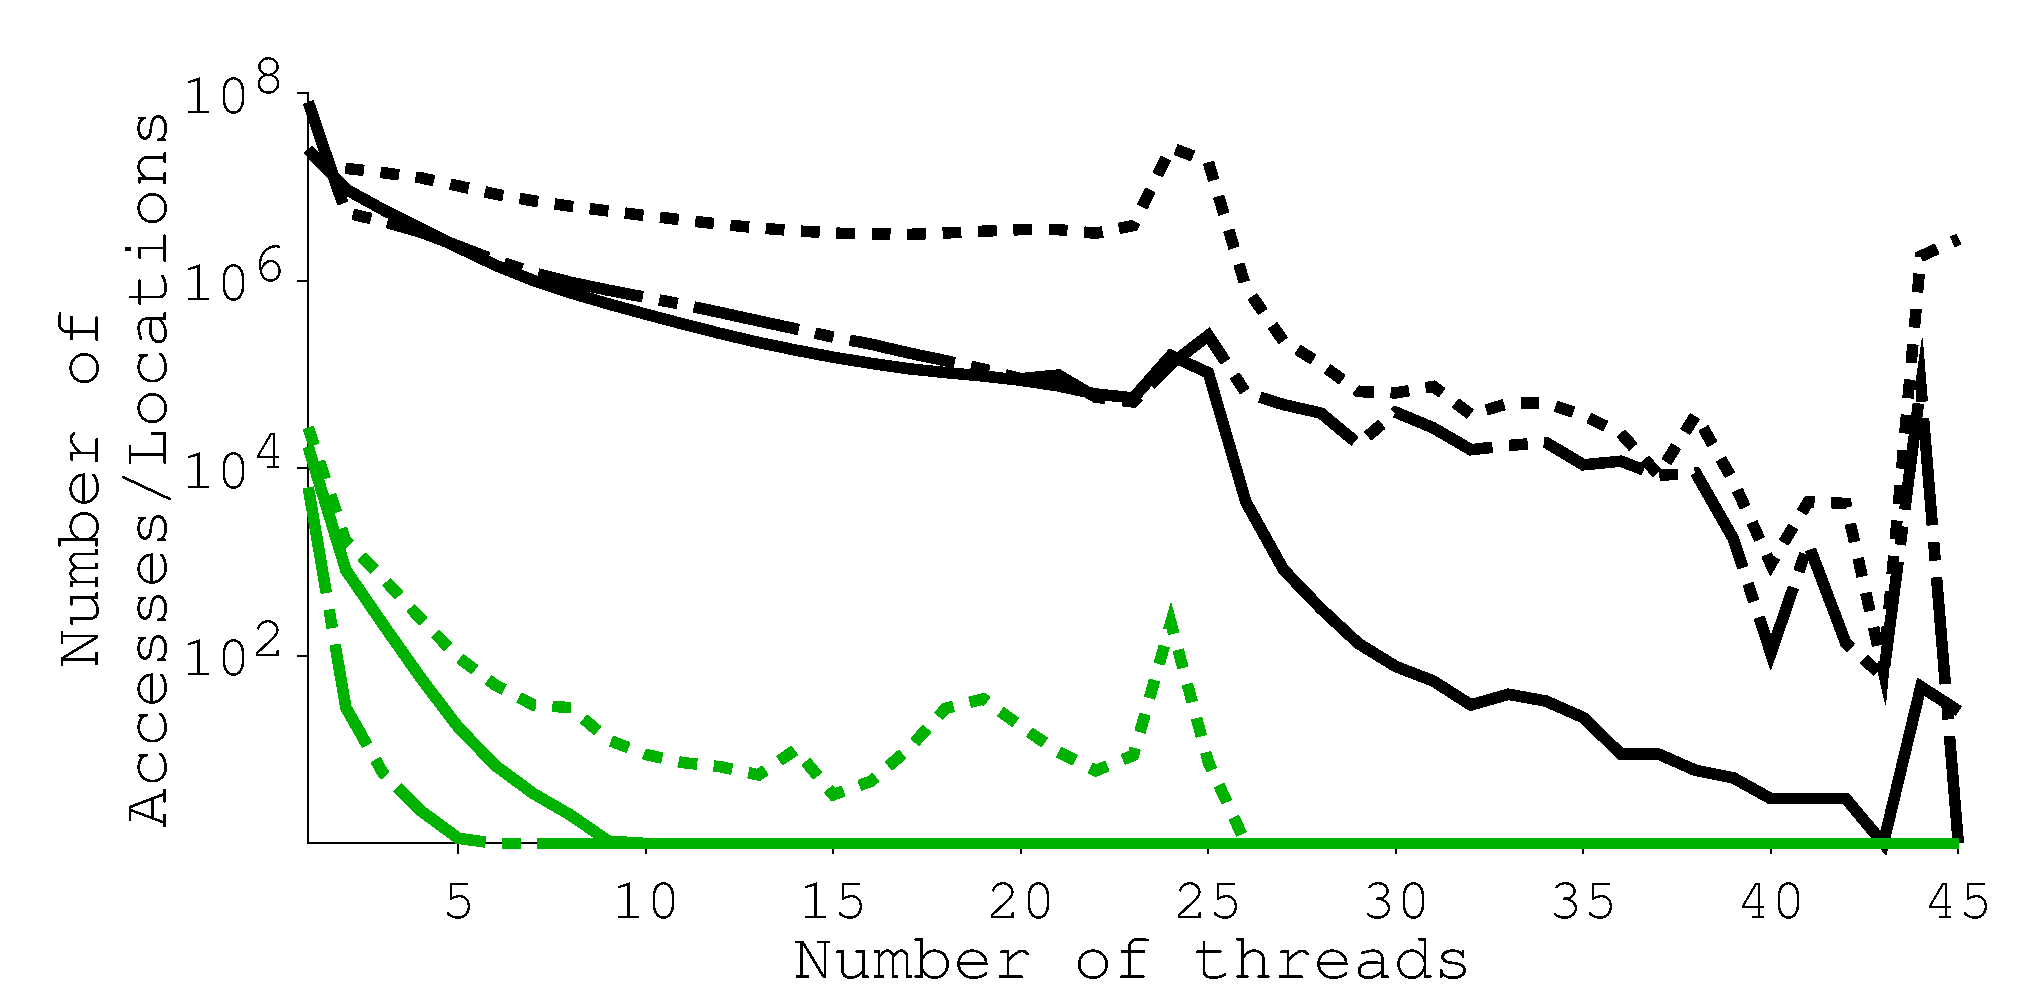
\includegraphics[width=\textwidth]{hotpot/Figures/g_plot_tensorflow_average.pdf}}
\caption[TensorFlow Sharing Analysis.]
{
TensorFlow Sharing Analysis.
Results of running a hand-writing recognition workloads provided by TensorFlow.
Black lines represent total amount of sharing.
Green lines represent sharing within five seconds.
}
\label{fig-tensorflow}
\end{center}
\end{figure}
}

Many large-scale datacenter applications require fast access to vast amounts of persistent data
and could benefit from \nvm's performance, durability, and capacity benefits.
For \nvm{}s to be successful in datacenter environments, they have to support these applications.
However, neither traditional distributed storage systems or DSM systems are designed for \nvm.
Traditional distributed storage systems~\cite{AdyaEtAl-Farsite,calder11-azure,DeCandia+07-Dynamo,Ghemawat03-GoogleFS,KubiEtAl00-Ocean,Petersen97-Bayou}
target slower, block-based storage devices.
Using them on \nvm{}s will result in excessive software and network overheads that outstrip \nvm's low latency performance~\cite{Zhang15-Mojim}.
DSM systems were designed for fast, byte-addressable memory, but lack the support for data durability and reliability.

Octopus~\cite{Octopus} is a recent RDMA-enabled distributed file system built for \nvm.
Octopus and our previous work Mojim~\cite{Zhang15-Mojim} are the only distributed \nvm-based systems that we are aware of.
Octopus was developed in parallel with \hotpot\ and has a similar goal as \hotpot: 
to manage and expose distributed PM to datacenter applications. 
However, Octopus uses a file system abstraction and is built in the user level.
These designs add significant performance overhead to native PM accesses (Section~\ref{sec:mongodb}).
Moreover, Octopus does not provide any data reliability or high availability, 
both of which are key requirements in datacenter environments.
